\documentclass[seminarskirad]{fer}


\usepackage{blindtext}
\usepackage{makecell}
\usepackage{listings}
\usepackage{xcolor}
\usepackage[utf8]{inputenc}
\usepackage[T1]{fontenc}

\lstset{
	basicstyle=\ttfamily\small,
	breaklines=true,
	breakatwhitespace=true,
	postbreak=\mbox{\textcolor{red}{$\hookrightarrow$}\space},
	columns=fullflexible,
	frame=single,
	backgroundcolor=\color{gray!10},
	literate=%
	{č}{{\v{c}}}1
	{ć}{{\'c}}1
	{ž}{{\v{z}}}1
	{š}{{\v{s}}}1
	{đ}{{\dj}}1
	{Č}{{\v{C}}}1
	{Ć}{{\'C}}1
	{Ž}{{\v{Z}}}1
	{Š}{{\v{S}}}1
	{Đ}{{\DJ}}1
}

%--- PODACI O RADU / THESIS INFORMATION ----------------------------------------

% Naslov na engleskom jeziku / Title in English
\title{Public transport traffic analysis}

% Naslov na hrvatskom jeziku / Title in Croatian
\naslov{Analiza prometa javnog gradskog prijevoza}

% Autor / Author
\author{Luka Miličević}

% Mentor 
\mentor{izv. prof. dr. sc. Ivana Bosnić}

% Datum rada na engleskom jeziku / Date in English
\date{may, 2025.}

% Datum rada na hrvatskom jeziku / Date in Croatian
\datum{svibanj, 2025.}

%-------------------------------------------------------------------------------


\begin{document}
\bibliographystyle{plain}

% Naslovnica se automatski generira / Titlepage is automatically generated
\maketitle


% Odovud započinje numeriranje stranica / Page numbering starts from here
\mainmatter


%--- SAŽETAK / ABSTRACT --------------------------------------------------------

% Sažetak na hrvatskom
\begin{sazetak}
  Seminar se bavi analizom prometa javnog gradskog prijevoza u stvarnom vremenu, temeljenom na podacima Zagrebačkog električnog tramvaja (ZET). Seminar se usredotočuje na prikupljanje i analizu podataka o vozilima javnog prijevoza, uključujući trenutačnu lokaciju vozila, vrijeme dolaska na stanice te uvjete na cesti i vremenske prilike. Podaci se prikupljaju u stvarnom vremenu putem API poziva, a zatim obrađuju kako bi se mogli koristiti za treniranje prediktivnog modela. Na temelju tih podataka, razvija se model za predviđanje vremena dolaska, koji se kontinuirano ažurira tijekom periodične batch obrade podataka. Seminar će istražiti osnovne koncepte i slična rješenja u industriji kroz prototipnu aplikaciju kojoj je cilj povećanje učinkovitosti i točnosti podataka kako bi korisnicima javnog prijevoza omogućio pravovremene i precizne informacije o dolasku vozila. 
\end{sazetak}

\begin{kljucnerijeci}
  Javni gradski prijevoz; Obrada u stvarnom vremenu; Prediktivni model; GTFS
\end{kljucnerijeci}


% Sadržaj se automatski generira / Table of contents is automatically generated
\tableofcontents


%--- UVOD / INTRODUCTION -------------------------------------------------------
\chapter{Uvod}
\label{pog:uvod}

U urbanim sredinama, javni gradski prijevoz ima ključnu ulogu u svakodnevnom životu građanina. On omogućuje efikasan i ekološki prihvatljiv način transporta velikog broja ljudi, smanjujući potrebu za individualnim vozilima, koje za posljedicu ima smanjenje prometnih gužvi i emisije štetnih plinova. Međutim, izazovi kao što su kašnjenja, nepouzdani rasporedi i nedostatak pravovremenih informacija umanjuju njegovu učinkovitost i privlačnost korisnicima.

Grad Zagreb u zadnjem izvješću bilježi značajan porast broja putnika u javnom prijevozu s obzirom na isto razdoblje prethodne godine. Prema podacima za 2024. godinu za razdoblje od srpnja do prosinca, ukupno je prevezeno 97,3 milijuna putnika, što je u usporedbi s istim razdobljem 2023. porast za 26,0\%, kada je prevezeno 77,2 milijuna putnika. Promatrajući cijelu godinu javnim gradskim prijevozom prevezen je ukupno 179,1 milijun putnika, što je 12,9\% više nego u 2023\cite{article4}.

\begin{figure}[htb]
	\centering
	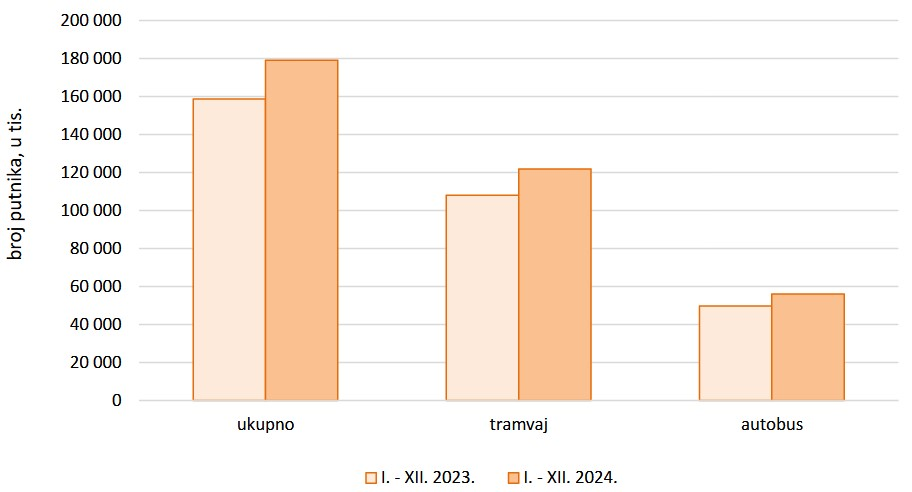
\includegraphics[width=0.9\linewidth]{Figures/graf-prijevoz.jpg} 
	\caption{Broj putnika javnog gradskog prijevoza grada Zagreba, siječanj - prosinac}
	\label{graf:prijevoz}
\end{figure}

Porast broja putnika moguće je djelomično pripisati nabavi rabljenih tramvaja te uvođenju novih niskopodnih tramvaja koje proizvodi tvrtka Končar, čime se povećava broj prijevoznih sredstava. Međutim, povećanje broja vozila i putnika ne bi trebao biti jedini strateški cilj ZET-a. Umjesto oslanjanja isključivo na kvantitativne pokazatelje potrebno je ulagati i u poboljšanje kvalitete usluge i iskustvo korisnika. Kako bi to ostvarili, ključno je osigurati pravovremene i točne informacije korisnicima koje će im omogućiti lakše i jednostavnije korištenje javnog prijevoza.

Ovaj seminar istražuje mogućnosti analize prometa u stvarnom vremenu te primjene umjetne inteligencije za razvoj prediktivnog modela kako bi se unaprijedilo pružanje informacija o dolasku vozila, čime bi se omogućilo učinkovitije planiranje i općenito bolja usluga za krajnje korisnike. Poseban naglasak stavljen je na korištenje otvorenih podataka Zagrebačkog električnog tramvaja (ZET) u kombinaciji s metodama strojnog učenja. U radu se također analiziraju relevantni istraživački radovi koji se bave sličnim temama\cite{article1}\cite{article2}\cite{article3}.

%-------------------------------------------------------------------------------
\chapter{Prikupljanje i obrada podataka}
\label{pog:prikupljanje}

Danas najčešće korišteni format za razmjenu podataka u industriji javnog prijevoza je GTFS (General Transit Feed Specification). GTFS je otvoreni format razvijen s ciljem omogućavanja standardizirane razmjene informacija o voznim redovima i rutama između pružatelja usluga javnog prijevoza i programera aplikacija. Nastao je kao rezultat suradnje između agencije za javni prijevoz TriMet iz Portlanda (Oregon, SAD) i Googlea. Cilj suradnje bio je razviti standardizirani i lako održiv format za prikaz podataka o javnom prijevozu unutar aplikacije Google Maps. Prvotno nazvan Google Transit Feed Specification, kasnije preimenovan u General Transit Feed Specification, danas predstavlja temelj digitalne infrastrukture mnogih sustava javnog prijevoza te je korišten u preko 10000 agencija i 100 zemalja diljem svijeta\cite{article5}.

Zagrebački električni tramvaj (ZET) jedna je od tih agencija, no njihova implementacija još se nalazi u ranoj fazi razvoja. ZET trenutačno koristi verziju 1.0 GTFS specifikacije, što znači da  sadrži osnovne informacije o voznim redovima i rutama, ali još uvijek nedostaju naprednije funkcionalnosti poput potpune integracije real-time podataka ili potpore za sve dodatne GTFS ekstenzije koje su dostupne u novijim verzijama. Unatoč toj činjenici i ovako djelomična implementacija GTFS-a omogućuje pristup ključnim informacijama potrebnim za analizu javnog prijevoza, posebno kada se kombiniraju s djelomično dostupnim real-time zapisima.

Pored GTFS podataka koji su temelj ovog seminara, koristit će se i podaci o vremenskim uvjetima, poput oborina i temperature, koji mogu utjecati na promet, kao i podaci o stanju na cestama, uključujući zastoje, nesreće i informaciju o protočnosti prometa. Uključivanjem ovih podataka u prediktivni model omogućuje bolju prilagodbu modela stvarnim uvjetima na terenu. Tradicionalni pristupi koji se oslanjaju isključivo na GTFS podatke pretpostavljaju da se vozila kreću prema voznom redu i u idealnim uvjetima, što u stvarnosti vrlo često nije slučaj.

\section{Opis podataka}
Kao što je već navedeno, koriste se GTFS podaci te podaci o vremenu i prometu.  
U nastavku su ukratko navedena glavna obilježja tih podataka:
\begin{enumerate}
	\item \textbf{GTFS podaci (General Transit Feed Specification)}\\
	Sastoje se od dva ključna dijela: \textbf{static i realtime}.\\
	\textbf{GTFS static} podaci obuhvaćaju minimalno šest CSV datoteka koje sadrže informacije o linijama, voznim redovima, stajalištima, putovanjima i drugim karakteristikama javnog prijevoza. Ove podatke održava i ažurira nadležna agencija u skladu s promjenama u voznim redovima ili zbog drugih operativnih potreba. U praksi se takva ažuriranja događaju tjedno ili mjesečno. Svaka GTFS static datoteka sadrži barem jedan ključni atribut (primarni ili strani ključ), čime se omogućuje međusobno povezivanje datoteka te rekonstrukcija logičkih odnosa između entiteta. Dijagram na slici \ref{slk:static} prikazuje jedan mogući raspored i spajanje GTFS datoteka u relacijski model.\\
	Neki od ključnih podataka sadržanih u GTFS static podacima su identifikatori linija, vozila i pojedinih putovanja; nazivi linija i stanica; raspored očekivanih odlazaka i dolazaka; redoslijed postaja na liniji; geometrija puta i tako dalje.
	
	\begin{figure}[htb]
		\centering
		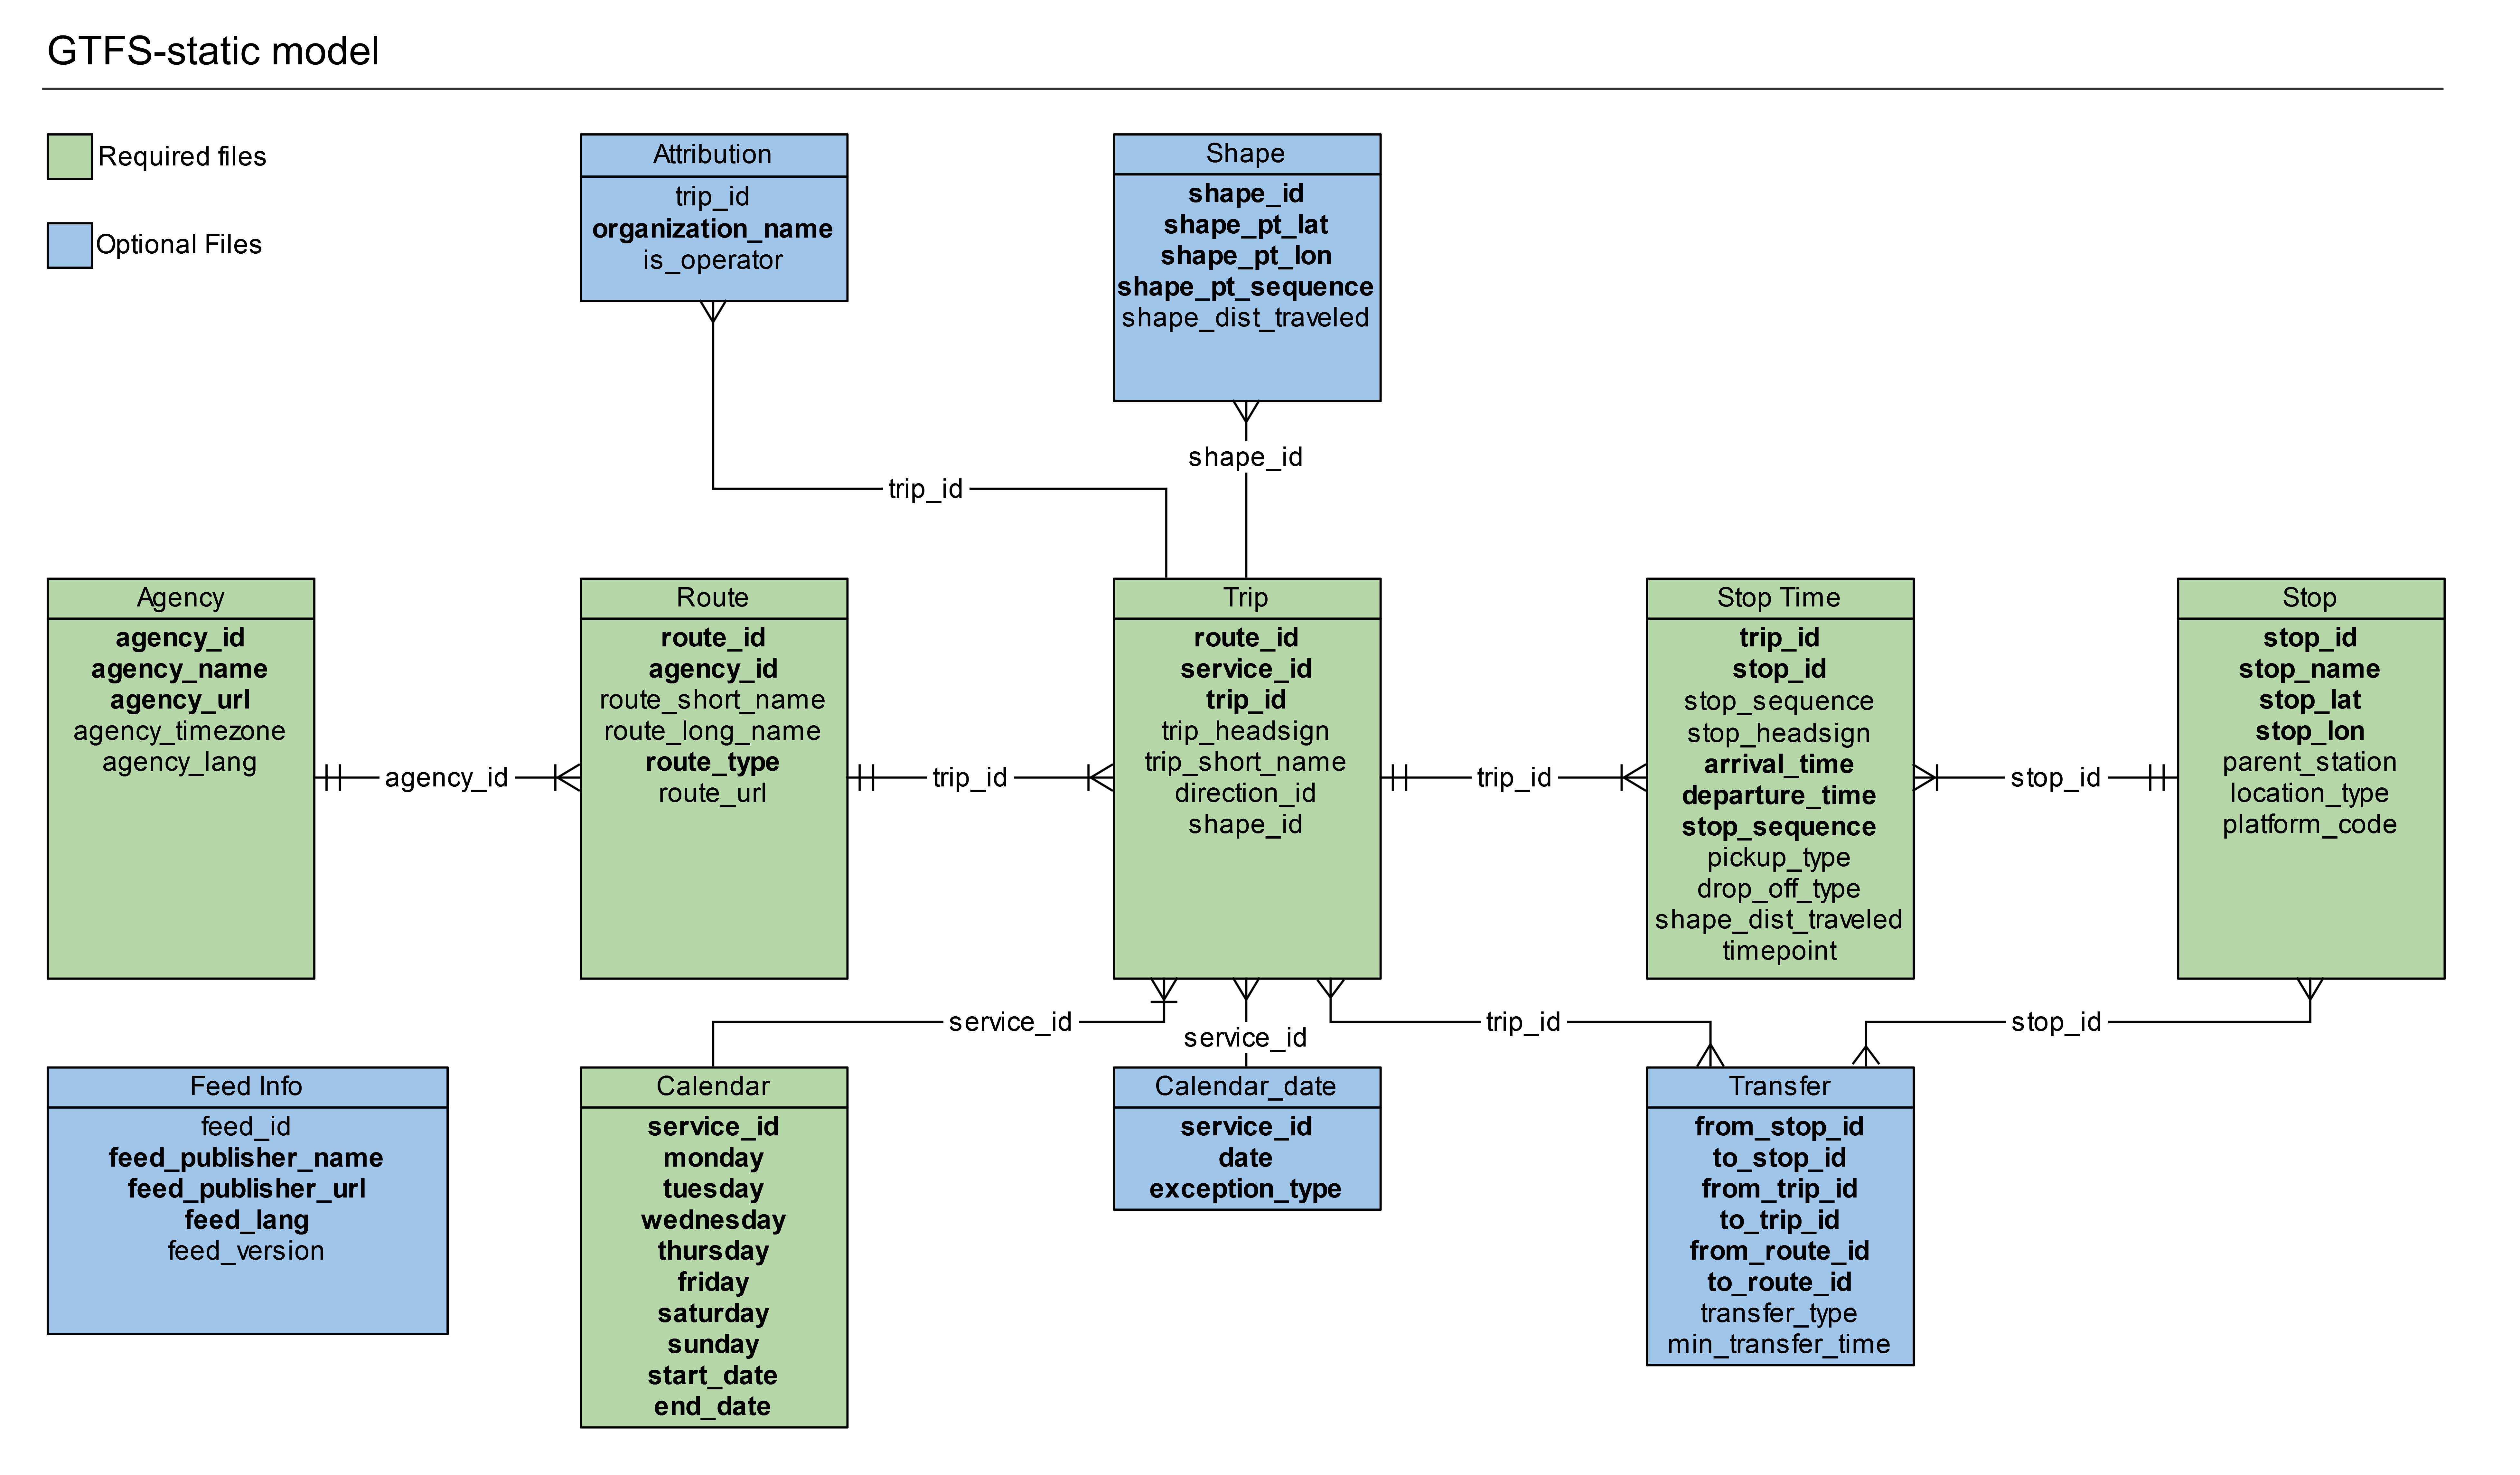
\includegraphics[width=0.9\linewidth]{Figures/gtfs-model.png} 
		\caption{Primjer GTFS static relacijskog modela}
		\label{slk:static}
	\end{figure}
	
	\textbf{GTFS realtime} podaci omogućuju praćenje javnog prijevoza u stvarnom vremenu. Sadrži informacije o geografskoj lokaciji vozila, statusu pojedinog putovanja poput vremena dolaska na pojedinu stanicu, kašnjenje u odnosu na raspored te obavijesti o mogućim poremećajima u prometu ili izmjenama u voznom redu. Oni također sadrže identifikatore koji omogućuju njihovo povezivanje s GTFS static podacima. Glavna prednost GTFS realtime podataka je korištenje formata Protocol Buffers (Protobuf). Protocol Buffers su jezično i platformski neutralni binarni format za serijalizaciju podataka. Dizajnirani su s ciljem brze obrade i minimalne veličine podataka (minimalan overhead) koji omogućuju učinkovito kodiranje, dekodiranje i prijenos podataka.
	
	\item \textbf{Vremenski podaci}\\
	Seminar će koristiti vremenske podatke poput temperature, tlaka, brzine vjetra te, najvažnije, podatke o vrsti i količini oborina, kako bi se ispitalo imaju li ti čimbenici utjecaj na odstupanja u voznom redu, iako je prethodno istraživanje Rashvand i sur. (\cite{article1}) pokazalo da vremenski uvjeti nemaju značajan utjecaj na pogrešku predviđanja dolazaka. Kao izvor podataka koristit će se podaci OpenWeatherMap API-ja, budući da nudi veću pokrivenost i detaljnije vremenske informacije u odnosu na Državni hidrometeorološki zavod (DHMZ).
	
	\item \textbf{Podaci o stanju u prometu}\\
	Podaci o stanju u prometu mogu imati značajan utjecaj na odstupanja u voznom redu, stoga će se razmatrati informacije o trenutačnoj brzini prometa, brzini prometa kada nema zagušenja te podaci o zastoju. Seminar će koristiti prometne podatke dobivene od TomTom-a, koji je odabran zbog svoje jednostavnosti korištenja i količine besplatnih API poziva. Alternativni izvori podataka mogu biti Google Maps Traffic API, koji je jedan od najpreciznijih i najopsežnijih izvora prometnih informacija, no njegova je uporaba ograničena zbog relativno visokih troškova. Ostale opcije uključuju HERE Traffic API, Bing Traffic API te druge slične usluge koje nude detaljne podatke o stanju u prometu.
	
\end{enumerate}

\section{Obrada podataka}
\label{pog:obrada}
Kao što je već spomenuto, GTFS static i realtime podaci sadrže brojne ključne atribute (primarne i strane ključeve) koji omogućuju povezivanje podataka i predstavljaju temelj aplikacije. Prije nego što ih je moguće povezati, potrebno je napraviti nekoliko koraka pripreme podataka. U slučaju GTFS static podataka koji su odmah čitljivi bilo kojim uređivačem teksta, nije potrebna posebna pretvorba podataka. Ipak, radi jednostavnijeg korištenja i povezivanja podataka preporučuje se njihovo učitavanje u bazu podataka. U okviru ovog seminara korištena je PostgreSQL baza podataka, koja omogućuje jednostavan uvoz CSV datoteka kao tablica te pomoću SQL upita lako povezivanje i izdvajanje željenih informacija. Da bi se olakšao taj postupak ostvarena je skripta koja preuzima najsvježije podatke od ZET-a, raspakira ih te ih učitava u bazu podataka.\\
GTFS realtime podaci zahtijevaju dodatni korak pretvorbe prije nego što ih je moguće učinkovito koristiti. Razlog tome, kako je ranije spomenuto, jest format Protocol Buffers koji je binarni format nečitljiv bez prethodnog dekodiranja. Korištenje binarnog formata u odnosu na tekstualne formate poput JSON-a ili XML-a donosi svoje prednosti poput zauzimanja znatno manje memorije za prijenos istih podataka (ostvaruje manji overhead) što rezultira bržim prijenosom podataka preko mreže, smanjuje kašnjenje podatka i opterećenje mreže. Jedini značajni nedostatak je potreba za kodiranjem i dekodiranjem podataka za ostvarenje prijenosa, što zahtijeva posebni alat ili biblioteku te odgovarajući opis podataka kako bi taj postupak bio uspješan. U praksi to ne predstavlja veliki problem, budući da je jedan od osnovnih principa pri dizajnu Protocol Buffersa bila neovisnost o korištenoj platformi i programskom jeziku tako da danas postoji široka podrška za najpopularnije programske jezike. Seminar pomoću odgovarajuće biblioteke lako obavlja kodiranje/dekodiranje podataka te ih je tada moguće učinkovito koristiti. Na slikama \ref{fig:code1} i \ref{fig:code2} prikazan je rezultat dekodiranja ZET-ovih GTFS realtime podataka.

\begin{figure}[h!]
	\centering
	\begin{minipage}{0.48\textwidth}
		\centering
		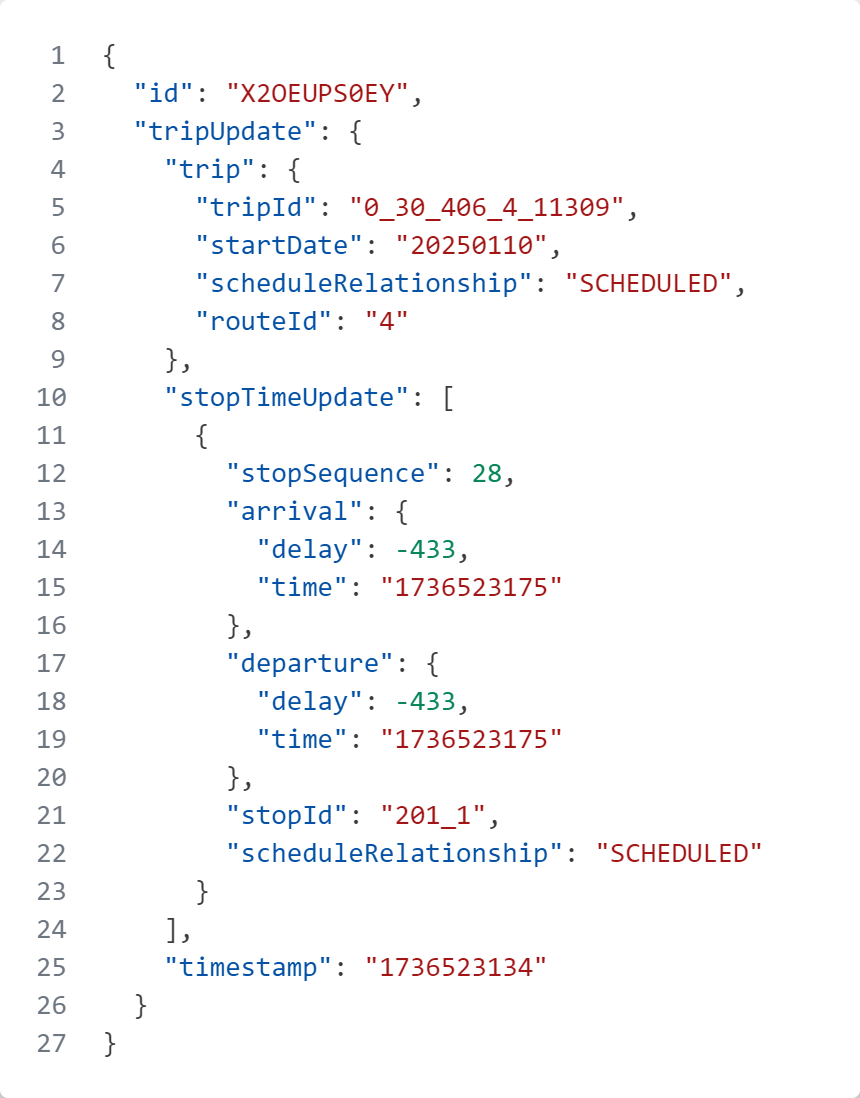
\includegraphics[width=\textwidth]{Figures/code.png}
		\caption{GTFS realtime podaci o statusu putovanja}
		\label{fig:code1}
	\end{minipage}
	\hfill
	\begin{minipage}{0.48\textwidth}
		\centering
		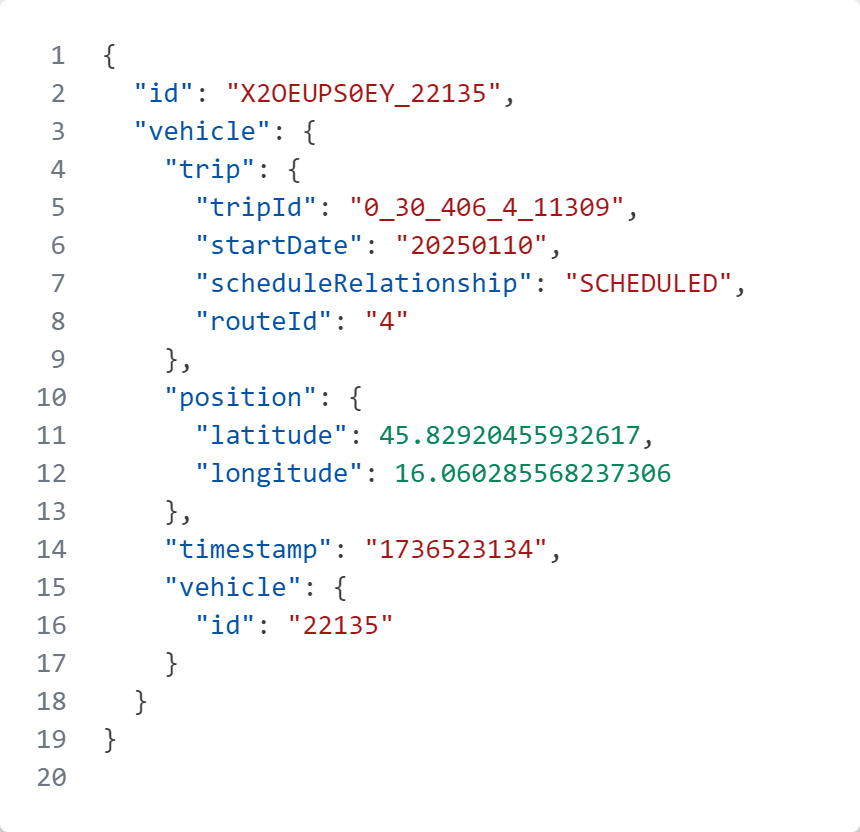
\includegraphics[width=\textwidth]{Figures/code2.png}
		\caption{GTFS realtime podaci o vozilu}
		\label{fig:code2}
	\end{minipage}
\end{figure}

Nakon što su ti koraci obavljeni, aplikacija će izvući podatke od značaja, poput identifikatora putovanja, broja rute, potvrđenog dolaska na posljednju stanicu (uključujući vrijeme i redni broj stanice) te identifikatora poruke. Potreba za identifikatorom poruke proizlazi iz činjenice da GTFS realtime podaci sadrže dva tipa poruka: poruku o statusu putovanja i poruku o podacima o vozilu. Tako se pomoću identifikatora poruke dohvaćaju podaci o trenutnoj lokaciji vozila za pojedino putovanje.\\
Na prikupljene podatke o putovanju i vozilu nadodaju se podaci o stanju u prometu i vremenski podaci na način da se preuzmu podaci od najbliže točke koja se koristila za mjerenje. Način odabira te točke bit će ukratko objašnjen u nastavku. Ti privremeni podaci predstavljaju jedno nezavršeno putovanje koje aplikacija sprema u radnu memoriju koristeći map strukturu podataka, gdje je ključ identifikator putovanja, što omogućuje brzo pretraživanje i pristup podacima. Oni se zadržavaju u memoriji onoliko dugo koliko je potrebno da bi pristigla poruka o dolasku vozila na sljedeću stanicu, odnosno kraj promatranog segmenta putovanja. Drugim riječima, najprije se bilježe podaci o dolasku tramvaja na početnu stanicu (vrijeme dolaska, broj stanice) i njegova trenutna lokacija. Na te se podatke nadodaju informacije o prometu i vremenskim uvjetima, kao i izračunata udaljenost do ciljne (sljedeće) stanice. Svi ti podaci se privremeno čuvaju u memoriji dok ne pristigne poruka o dolasku tramvaja na sljedeću stanicu. Taj proces se izvodi u beskonačnoj petlji.\\
Kada je prikupljen određen broj podataka o završenim putovanjima, aplikacija prebacuje podatke iz radne memoriju u perzistentnu memoriju, odnosno bazu podataka gdje se čuvaju i čekaju obrađivanje unutar neuronske mreže.\\

Odabir točaka za mjerenje, odnosno lokacija nad kojima se izvršavaju upiti o vremenskim uvjetima i prometnoj situaciji, temelji se na GTFS static podacima i bit će objašnjen na primjeru sa slika \ref{slk:odabrane} i \ref{slk:odabrane-zoom}. Na početku je potrebno definirati promatrane rute (npr. linije 5, 17, 109, 13, 3) te se za njih uz pomoć \textit{trips.txt} i \textit{shapes.txt} pronađu sve moguće geometrije puta (putanje). Putanje se potom uzorkuju svakih 500 metara te nastaju kandidatne točke  (crvene točke), koje se zatim zbog preklapanja i blizine s drugim kandidatima grupiraju pomoću algoritma za grupiranje točaka s obzirom na udaljenost. Izlaz algoritma su reprezentativne točke (žute točke) koje će biti korištene za upite o stanju prometa. Razlog grupiranja je vrlo jednostavan, a to je smanjenje potrebnih API poziva, jer je moguće da su neke točke međusobno jako blizu te će stanje u prometu za njih biti gotovo jednako (Slika \ref{slk:odabrane-zoom}). Tako za primjer u kojemu su promatrane linije 5, 17, 109, 13, 3 na početku postoji 640 kandidatnih točaka, provedbom algoritma grupiranja taj broj se smanjuje na 222 točke.\\
Za točke koje će se koristiti u upitima o vremenskim uvjetima potrebno je napraviti još jedan korak – optimizaciju kojom se dodatno smanjuje broj potrebnih API poziva. S obzirom na to da područje grada Zagreba nije značajno podložno mikroklimatskim razlikama, moguće je grupirati prostorno bliske točke i koristiti jednu zajedničku vremensku prognozu za sve njih. U tu svrhu nad kartom grada Zagreba konstruira se mreža sastavljena od kvadrata dimenzija 1×1 kilometar. Ako se unutar pojedinog kvadrata nalazi barem jedna odabrana točka (žuta točka), središte tog kvadrata odabire se kao reprezentativna točka za vremenski upit. Tako se za isti primjer kao prije, od 222 odabrane točke, broj smanjuje na samo 38 točaka.

\begin{figure}[h]
	\centering
	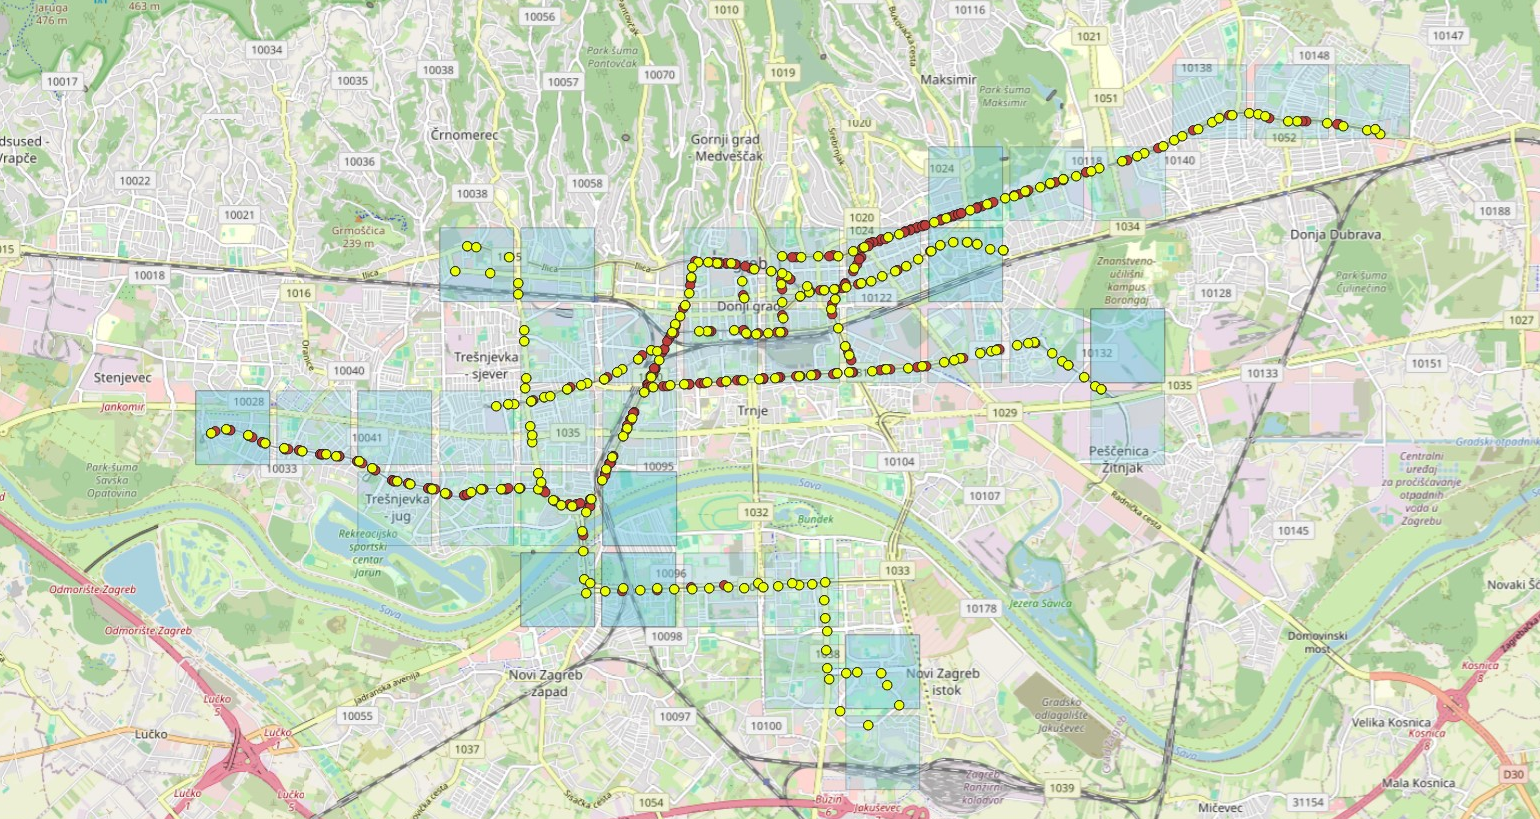
\includegraphics[width=0.8\textwidth]{Figures/odabrane-tocke.png}
	\caption{Odabrane točke za mjerenja}
	\label{slk:odabrane}
	
	\vspace{1em}
	
	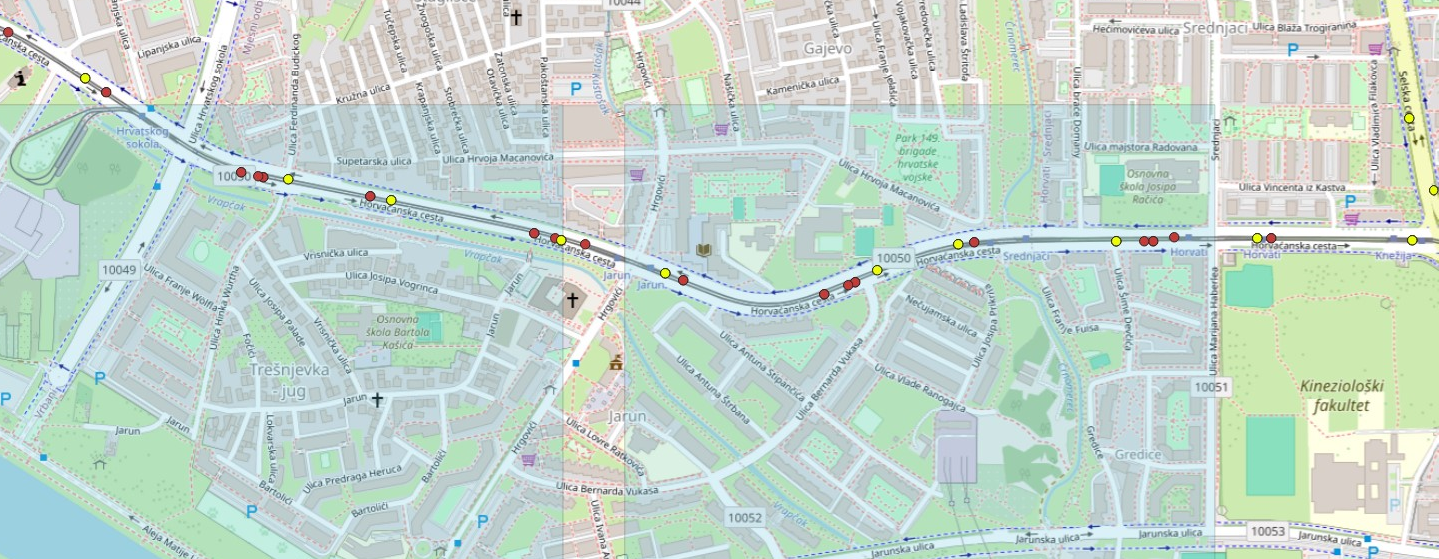
\includegraphics[width=0.8\textwidth]{Figures/odabrane-tocke-zoom.png}
	\caption{Uvećana slika kojom je uočljivo grupiranje}
	\label{slk:odabrane-zoom}
\end{figure}


%-------------------------------------------------------------------------------
\chapter{Prediktivni model}
\label{pog:prediktivni}
Istraživački radovi  koji su poslužili kao nadahnuće za ovaj rad pokazali su da metode strojnog učenja, a posebno neuronske mreže, predstavljaju trenutno najučinkovitiji pristup za predviđanje vremena dolaska vozila javnog prijevoza u stvarnim uvjetima. U usporedbi s tradicionalnim metodama poput regresijskih modela ili modela podrške vektorima (SVM), neuronske mreže bolje se nose s nelinearnostima, vremenskom ovisnošću i višedimenzionalnim značajkama koje su prisutne u ulaznim podacima\cite{article1}\cite{article2}.

U istraživanju kojeg su proveli Rashvand i sur. (\cite{article1}), korištenjem potpuno povezane neuronske mreže (FCNN), postignuta je prosječna pogreška predikcije (RMSE) od 35,74 sekunde, što znači da je predviđeno vrijeme dolaska autobusa u prosjeku imalo odstupanje manje od 36 sekundi na skupu podataka iz New Yorka koji uključuje 200 linija autobusa i 2 milijuna ulaznih točaka. S druge strane, C. Fors Johansson koristio je naprednu metodu neuronske mreže, Long Short-Term Memory (LSTM), koja omogućava dugoročno pamćenje informacija i učenje zavisnosti između podataka tijekom vremena, čime postiže preciznija predviđanja. Primjenom LSTM-a za prepoznavanje zavisnosti između pojedinih stanica na liniji prijevoza, uspio je ostvariti čak 63,7\% predviđanja unutar okvira od \textpm1 minute\cite{article3}.

S obzirom na sličnost problema s prethodno navedenim radovima, u ovom seminaru primijenit će se pristup temeljen na neuronskim mrežama s ciljem izgradnje modela koji može uzimati u obzir podatke o prometu i ostale varijabilne značajke te isporučivati točne informacije o očekivanom dolasku vozila. U nastavku će biti detaljno opisane korištene metode, arhitektura neuronske mreže, način treniranja modela te evaluacija njegove točnosti.

\section{Neuronska mreža}
\label{pog:neuronska}
"Neuronska mreža jest skup međusobno povezanih jednostavnih procesnih elemenata, jedinica ili čvorova, čija se funkcionalnost temelji na biološkom neuronu. Pri tome je obradbena moć mreže pohranjena u snazi veza između pojedinih neurona tj. težinama do kojih se dolazi postupkom prilagodbe odnosno učenjem iz skupa podataka za učenje."
(Dalbelo Bašić, Čupić i Šnajder \cite{ferumjetne}). \\Drugim riječima neuronske mreže su pojednostavljeni matematički model ljudskog mozga u kojem se podaci obrađuju s pomoću neurona (čvorova) povezanih vezama različite težine (jakost). Svaki neuron prima ulazne podatke, obrađuje ih i primjenjuje aktivacijsku funkciju (prijenosnu funkcija) te izlaz prosljeđuje dalje.

\begin{figure}[htb]
	\centering
	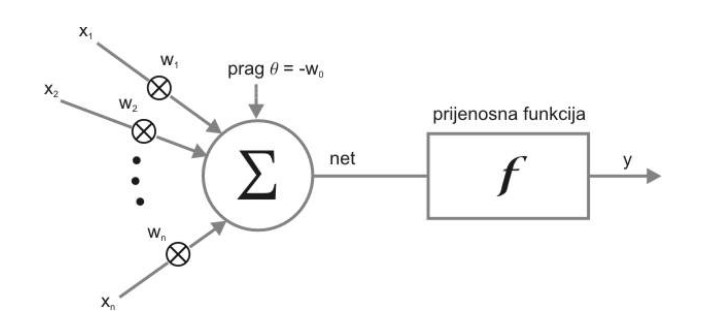
\includegraphics[width=0.65\linewidth]{Figures/neuron.jpg} 
	\caption{Umjetni neuron \cite{ferumjetne}}
	\label{slk:neuron}
\end{figure}

Neuronska mreža ima sposobnost učenja, to jest ima sposobnost prilagođavanja svojih težina kako bi smanjila pogrešku između stvarnog i očekivanog izlaza. Zbog te sposobnosti, neuronske mreže odlično rješavaju probleme klasifikacije i predviđanja te imaju jako široku primjenu u rješavanju zadataka poput raspoznavanja uzoraka, aproksimacije funkcija, obrade slika, videozapisa i govora i raznih drugih problema u području umjetne inteligencije.\\
\pagebreak


Neuronska mreža je sastavljena od najčešće velikog broja međusobno povezanih neurona organiziranih u slojeve. Ti slojevi su:
\begin{itemize}
	\item \textbf{Ulazni sloj} - prima podatke iz vanjskog svijeta (nemaju funkcionalnost neurona, samo prosljeđuju podatke)
	\item \textbf{Skriveni sloj} - najčešće postoji više skrivenih slojeva koji zajedno vrše obradu podataka
	\item \textbf{Izlazni sloj} - daje krajnji rezultat neuronske mreže
\end{itemize}

\begin{figure}[htb]
	\centering
	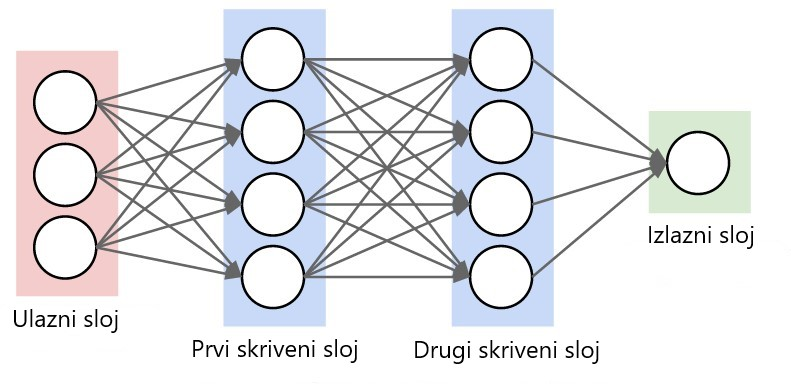
\includegraphics[width=0.56\linewidth]{Figures/neuronskaprimjer.jpg} 
	\caption{Slojevi neuronske mreže}
	\label{slk:neuronskaprimjer}
\end{figure}

Broj slojeva i neurona mreže, odnosno njena arhitektura utječu na performanse modela. Mreže s većom arhitekturom mogu se primijeniti na složenije zadatke, bolje prepoznati nelinearne veze te proučiti više značajki (ulazne informacije), ali su sklonije problemima poput prenaučenosti i zahtijevaju više računalnih resursa. Prenaučenost je pojam koji opisuje situaciju kada model tijekom treniranja previše prilagodi svoje parametre na podatke iz skupa za učenje. Posljedica toga, kada se model počne ispitivati na skupu podataka za testiranje koji predstavlja dosad neviđene podatke, točnost modela značajno opada. Manje neuronske mreže primjenjuju se na jednostavnije zadatke te su manje računalno zahtjevne i manje sklone prenaučenosti.

Prije samog učenja mreže, ulazni podaci se moraju normalizirati. Normalizacija sprječava velike razlike u rasponima vrijednosti pojedinih značajki, što može uzrokovati da velike vrijednosti dominiraju nad manjima. Primjenom normalizacije se uravnotežuje utjecaj značajki i smanjuje negativan utjecaj ekstremnih vrijednosti. Osim toga, normalizacija ubrzava proces učenja i doprinosi boljoj generalizaciji modela, smanjujući rizik od prenaučenosti. Dvije od najpopularnijih tehnika normalizacije su standardizacija numeričkih (brojčanih) značajki i "One-Hot Encoding". Standardizacija numeričkih značajki transformira značajke tako da imaju srednju vrijednost 0 i standardnu devijaciju 1, dok se "One-Hot Encoding" koristi za pretvorbu kategorijskih značajki u binarne vektore koje model može shvatiti.\\
Nakon što se obavi normalizacija ulaznih podataka, oni se dijele u dva skupa: skup za treniranje i skup za testiranje. Skup za treniranje koristi se tijekom procesa učenja, gdje neuronska mreža prilagođava svoje težine kako bi što bolje predviđala ishode na temelju ulaznih podataka. Moguće je dodatno razdijeliti ga na skup za treniranje i skup za validaciju. S druge strane, skup za testiranje koristi se nakon procesa učenja kako bi se evaluirala točnost modela nad dosad neviđenim podacima. Za evaluaciju točnosti modela se često koristi MAE (Mean absolute error) - srednja apsolutna pogreška. Ona se računa kao prosjek apsolutnih razlika između predviđenih i stvarnih vrijednosti te prikazuje prosječnu pogrešku. Pored MAE koriste se i MSE (Mean Squared Error) te RMSE (Root Mean Squared Error).\\

Proces učenja neuronske mreže se provodi algoritmom koji prilagođava težine veza između neurona s ciljem smanjenja pogreške između predviđenih i stvarnih podataka. Taj proces se ponavlja kroz više iteracija (epoha), dok mreža ne postigne zadovoljavajuću točnost. Ukratko, svaki neuron prima izlaze neurona iz prethodnog sloja s kojima je povezan, zatim ih sumira, dodaje pomak (bias) i na dobiveni rezultat primjenjuje aktivacijsku funkciju. Aktivacijska funkcija određuje izlaz neurona i omogućuje da izlaz nije samo linearna kombinacija ulaza. Izlaz neurona potom se šalje sljedećem sloju mreže. Nakon što se podaci propagiraju kroz sve slojeve, izračunava se ukupna pogreška modela. Tada se obavlja korigiranje težina te kod metode gradijentnog spusta korigiranje se provodi unatrag kroz mrežu — od izlaznog prema ulaznom sloju. 

\newpage
Kroz ovaj seminar proučene su četiri različite konfiguracije neuronskih mreža. Odabrane arhitekture razlikuju se po broju skrivenih slojeva i broju neurona po skrivenom sloju te primjenom dodatnih tehnika poput ranog zaustavljanja (early stopping), što omogućuje bolju generalizaciju i smanjenje prenaučenosti modela.
U Tablici \ref{tab:results} prikazani su rezultati treniranja za svaku od konfiguracija, uključujući metrike pogreške na skupu za učenje, validaciju i testiranje.

\begin{table}[htb]
	\centering
	\resizebox{\textwidth}{!}{
	\begin{tabular}{lcccc}
		\hline
		\textbf{Skriveni slojevi} & \textbf{64x32} & \textbf{128x64} & \textbf{320x200x100x40x5} & \makecell{\textbf{320x200x100x40x5} \\ \textbf{+ early stopping}}
		 \\
		\hline
		Training Loss (MSE)           & 1580.2980      & 1561.3629                     & 1115.0692                 & 973.2731                               \\
		Validation Loss (MSE)         & 1629.9922      & 1552.5287                     & 1352.4648                 & 1292.6776                              \\
		Training MAE (sekunde)        & 29.2435        & 29.0271                       & 24.1745                   & 22.5490                               \\
		Validation MAE (sekunde)      & 29.8322        & 28.8568                       & 26.1842                   & 25.3439                               \\
		Test MAE (sekunde)      & 29.11        & 28.15                       & 24.94                   & 24.27                              \\
		\hline
	\end{tabular}	
	}
	\caption{Rezultati treniranja neuronskih mreža za različite konfiguracije}
	\label{tab:results}
\end{table}

Analizom rezultata prikazanih u tablici vidljivo je da povećanje složenosti arhitekture neuronske mreže dovodi do smanjenja pogreške. Najjednostavnija konfiguracija, sastavljena od dva skrivena sloja (64x32), ostvarila je najveće vrijednosti pogrešaka na svim skupovima podataka. Dodavanjem dodatnih slojeva i povećanjem broja neurona značajno su poboljšane performanse modela, što je vidljivo kroz smanjenje vrijednosti MSE i MAE metrika. Najbolje rezultate postigla je mreža sačinjenja od pet skrivenih slojeva (320x200x100x40x5), preuzeta iz rada Rashvanda i suradnika (\cite{article1}), nad kojom je dodatno primijenjena tehnika ranog zaustavljanja (early stopping). Ova konfiguracija ostvarila je najniže pogreške nad skupovima za treniranje, validaciju i testiranje te je odabrana kao referentni primjer za koji će biti prikazani grafovi rezultata učenja.


\begin{figure}[htb]
	\centering
	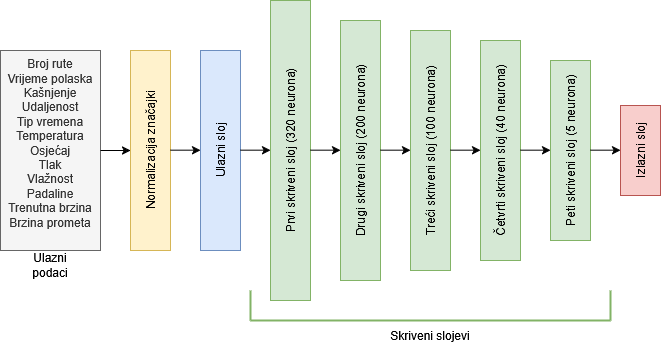
\includegraphics[width=0.75\linewidth]{Figures/mreza.png} 
	\caption{Odabrana struktura mreže}
	\label{slk:mreza}
\end{figure}

%-------------------------------------------------------------------------------
\chapter{Prototipna aplikacija}
\label{pog:prototip}

Iako je prototipna aplikacija djelomično predstavljena u ranijim poglavljima, u nastavku slijedi sažeti prikaz njezine funkcionalnosti kako bi se pružio jasan pregled rada aplikacije.\\

\begin{figure}[htb]
	\centering
	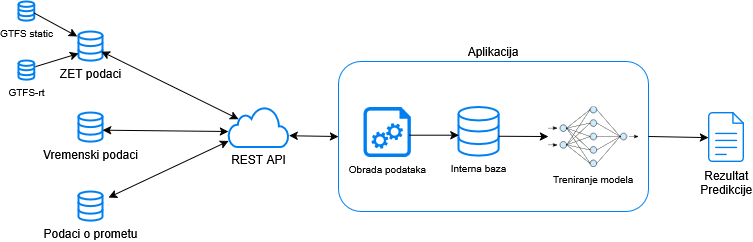
\includegraphics[width=0.9\linewidth]{Figures/sustav.png} 
	\caption{Sažeti pregled sustava}
	\label{slk:sustav}
\end{figure}

Na dijagramu na slici \ref{slk:sustav} prikazan je pogled na sustav s visoke razine. Aplikacija pomoću REST API sučelja i odgovarajućih metoda dohvaća podatke iz tri izvora:
\begin{itemize}
	\item GTFS podaci sa službene stranice ZET-a
	\item Vremenski podaci preuzeti s platforme OpenWeatherMap
	\item Podaci o prometu preuzeti s TomTom
\end{itemize}
Usluge OpenWeatherMap i TomTom odabrane su zbog jednostavnosti korištenja te dovoljnog broja besplatnih API poziva za izradu ovog seminara. U slučaju daljnjeg razvoja aplikacije preporučljivo je razmatranje alternativnih opcija za dohvaćanje podataka o stanju prometa poput Google Maps API, koji može ponuditi veću preciznost i skup podataka.

Obrada podataka provodi se prema postupku opisanom u poglavlju \ref{pog:obrada}. Nakon obrade, podaci se pohranjuju u internu bazu podataka implementiranu u PostgreSQL-u. Baza sadrži tablicu promatranja koja se koristi kao ulaz za treniranje neuronske mreže. Proces treniranja modela moguće je pokrenuti ručno ili automatizirati kada se prikupi dovoljno podataka (batch obrada). U oba slučaja, podaci se najprije dohvaćaju iz baze podataka, zatim se nad njima provodi normalizacija i podjela na skupove za treniranje, validaciju i testiranje, nakon čega slijedi proces učenja neuronske mreže koji je opisan u poglavlju \ref{pog:neuronska}. U istom poglavlju prikazana je i odabrana arhitektura mreže.
Istrenirani model moguće je spremiti kako bi se u budućnosti mogao koristiti za izvođenje predikcija. Za predikciju vremena dolaska tramvaja potrebno je unijeti trenutačnu lokaciju tramvaja, trenutačno vrijeme te stanje na cesti

\section{Rezultati}
Kao što je već navedeno u poglavlju \ref{pog:neuronska}, rezultati i grafovi temelje se na odabranoj neuronskoj mreži sa strukturom skrivenih slojeva 320x200x100x40x5 neurona. 

Treniranje je provedeno na skupu od N = 36687 ulaznih podataka prikupljenih tijekom vremenskog razdoblja od pet dana. Od toga, 75 \% podataka koristi se za trening i validacijski skup, dok je preostalih 25 \% rezervirano za testni skup. Unutar skupa za treniranje, 10 \% podataka izdvojeno je kao validacijski skup.
\begin{figure}[htb]
	\centering
	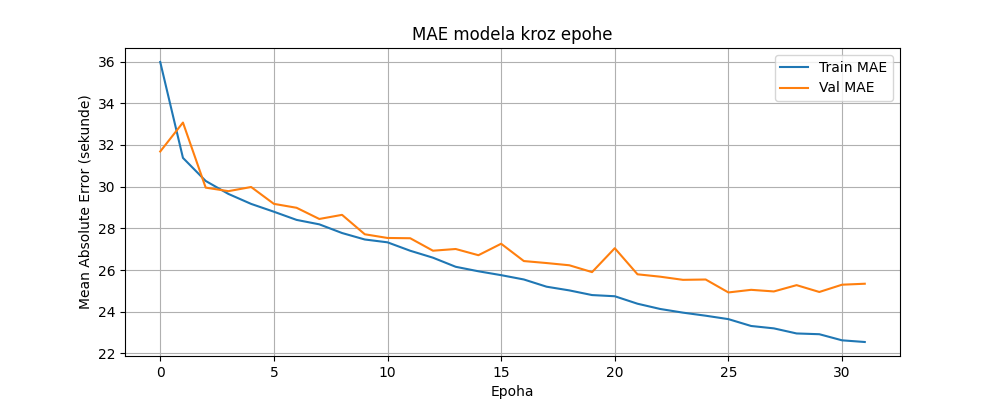
\includegraphics[width=0.8\linewidth]{Figures/mae_epoha.png}
	\caption{Prosječna pogreška treniranja kroz epohe}
	\label{fig:mae_epoha}
\end{figure}
Krivulja prosječne greške tijekom treniranja na početku brzo opada, a zatim se pad usporava, što je tipično za neuronske mreže.
\newpage

U nastavku je prikazan isječak konkretnih ispisa predikcija modela za neke testne primjere uspoređeni sa stvarnim vremenima dolaska.
\begin{lstlisting}
Tramvaj 5 je krenuo sa stanice 22 u 15:34:43, očekivano vrijeme dolaska na narednu stanicu 23 je 15:37:14, stvarno vrijeme dolaska 15:36:35
Tramvaj 4 je krenuo sa stanice 5 u 16:21:07, očekivano vrijeme dolaska na narednu stanicu 6 je 16:22:11, stvarno vrijeme dolaska 16:22:14
Tramvaj 17 je krenuo sa stanice 15 u 17:36:22, očekivano vrijeme dolaska na narednu stanicu 16 je 17:37:29, stvarno vrijeme dolaska 17:37:27
\end{lstlisting}

Ako promotrimo sve testne primjere i njihove pogreške izražene u sekundama, možemo ih vizualizirati pomoću histograma koji prikazuje raspodjelu pogrešaka modela \ref{fig:histogram}. Histogram poprima oblik približan normalnoj (Gaussovoj) distribuciji, što ukazuje da većina testnih primjera poprima malu pogrešku. Točnije, ispis modela prikazuje i postotak testnih primjera koji pripadaju određenom rasponu mjerenog od stvarnog vremena dolaska, pri čemu su rezultati:
\begin{itemize}
	\item Rasponu od ±10 sekundi od stvarnog dolaska pripada 30.61\% testnih primjera
	\item Rasponu od ±30 sekundi od stvarnog dolaska pripada 70.91\% testnih primjera
	\item Rasponu od ±60 sekundi od stvarnog dolaska pripada 92.85\% testnih primjera
	\item Rasponu od ±120 sekundi od stvarnog dolaska pripada 99.26\% testnih primjera
\end{itemize}

\begin{figure}[htb]
		\centering
		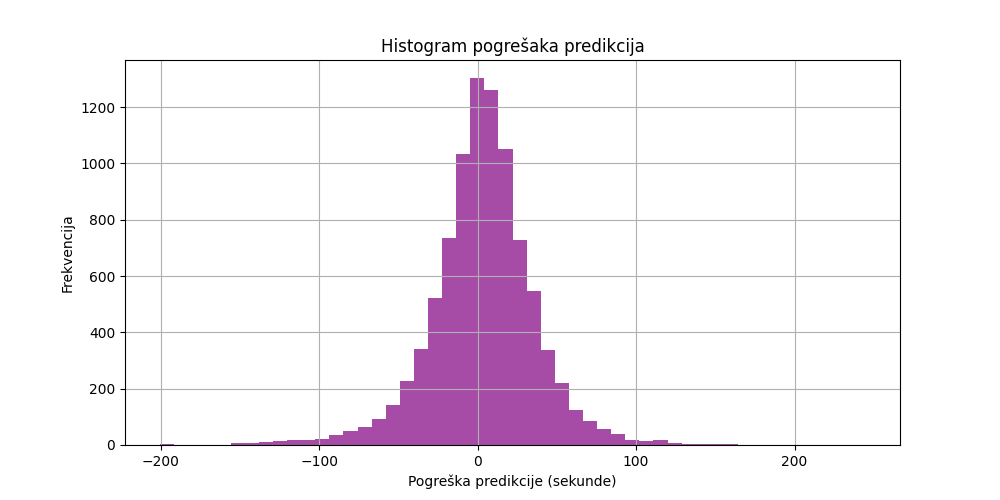
\includegraphics[width=0.8\linewidth]{Figures/histogram.png}
		\caption{Histogram pogrešaka predikcije}
		\label{fig:histogram}
\end{figure}

Vrijednosti su vrlo dobre ako ih usporedimo s istraživanjem C. Fors Johanssona, koji je primjenom LSTM modela za prepoznavanje zavisnosti između stanica na liniji prijevoza ostvario 63,7\% predviđanja unutar okvira od \textpm1 minute \cite{article3}.
Međutim, treba imati na umu da se rezultati ne bi trebali shvaćati previše ozbiljno zbog ograničenosti skupa podataka — korišteno je samo 36687 primjera prikupljenih tijekom 5 dana, u kojima nije bilo značajnih odstupanja u vremenu i prometu.

Pored histograma na slikama \ref{fig:postotna_pogreska} i \ref{fig:predvideno_stvarno} prikazana su dva grafa koji također vizualno prikazuju pogrešku testnih primjera.

\begin{figure}[h!]
	\centering
	\begin{minipage}{0.48\textwidth}
		\centering
		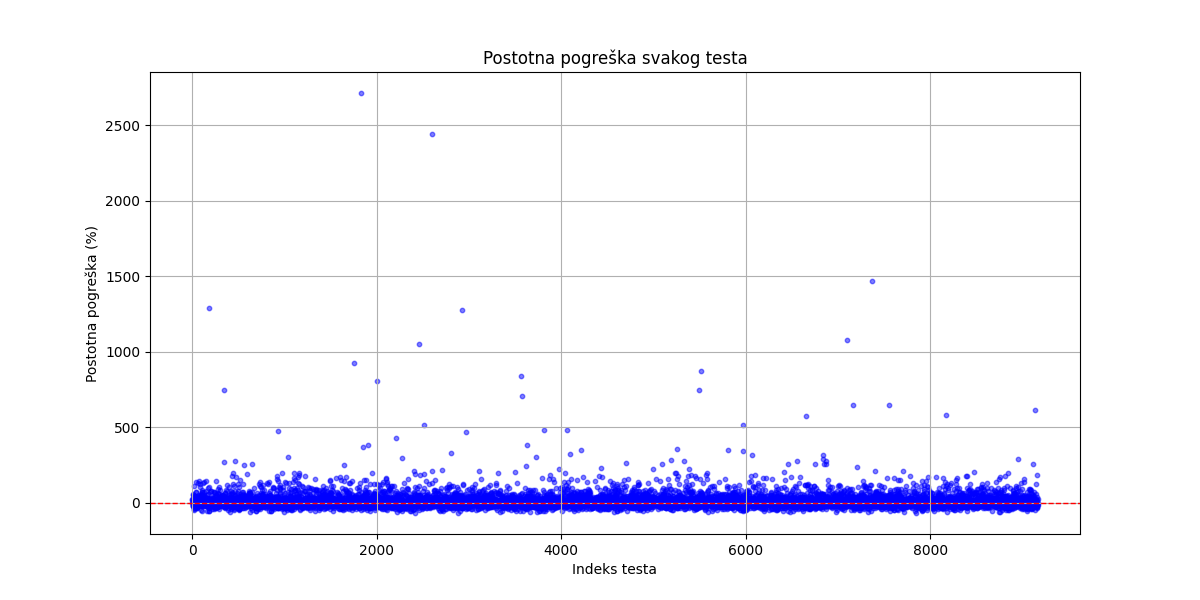
\includegraphics[width=\textwidth]{Figures/postotna_pogreska.png}
		\caption{Postotna pogreška testnih primjera}
		\label{fig:postotna_pogreska}
	\end{minipage}
	\hfill
	\begin{minipage}{0.48\textwidth}
		\centering
		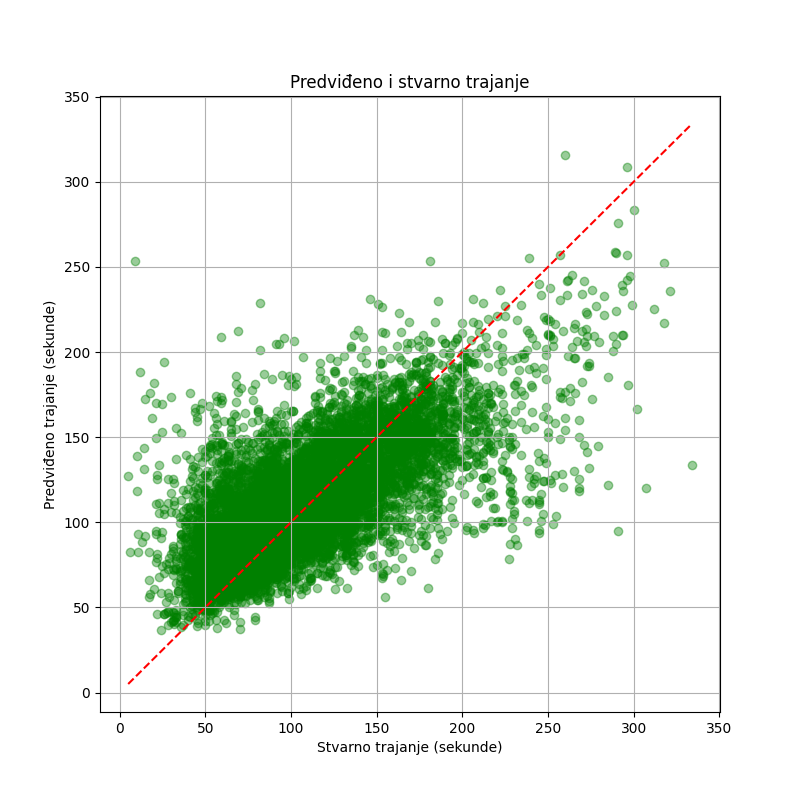
\includegraphics[width=\textwidth]{Figures/predvideno_stvarno.png}
		\caption{Ovisnost predviđenog vremena trajanja puta i stvarnog trajanja}
		\label{fig:predvideno_stvarno}
	\end{minipage}
\end{figure}

Zanimljivo je proučiti graf na slici \ref{slk:korelacije_znacajki}, koji prikazuje korelacijsku matricu svih značajki te omogućuje bolji uvid u međusobne odnose među podacima. Za vremenske značajke temperatura i osjećaj (feels\_like temperatura) može se zaključiti da su u gotovo savršenoj korelaciji, što upućuje na to da jedna od njih nije nužna za treniranje modela. Također se može primijetiti da je temperatura u obrnutoj korelaciji s tlakom i vlagom, dok tlak i brzina vjetra pokazuju obrnutu korelaciju, što je u skladu s prirodnim zakonitostima, ali nema značajan utjecaj na model. Općenito vremenske značajke nemaju značajan utjecaj na predikcije modela što je vidljivo na grafu \ref{fig:korelacije_vrijeme} te je u skladu s tvrdnjom istraživanja Rashvand i sur. (\cite{article1}) da vremenski uvjeti nemaju značajan utjecaj na pogrešku predviđanja dolazaka.
Daljnjim proučavanjem matrice korelacija može se primijetiti da najveći utjecaj na pogrešku predviđanja dolazaka ima udaljenost (korelacija od 0.4) te brzina kretanja (korelacija od -0.08), što je u skladu s očekivanjima, budući da veća udaljenost i niža brzina doprinose dužem trajanju putovanja.

\begin{figure}[htb]
	\centering
	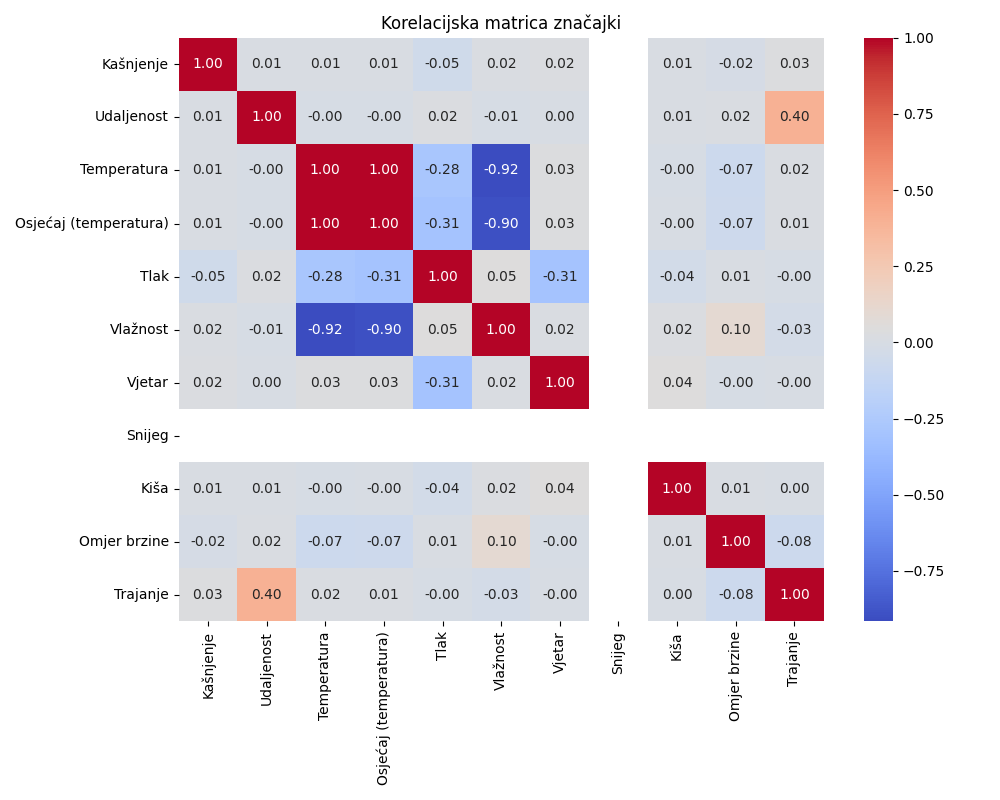
\includegraphics[width=0.9\linewidth]{Figures/korelacija_znacajki.png} 
	\caption{Matrica korelacija značajki}
	\label{slk:korelacije_znacajki}
\end{figure}

\begin{figure}[h!]
	\centering
	\begin{minipage}{0.48\textwidth}
		\centering
		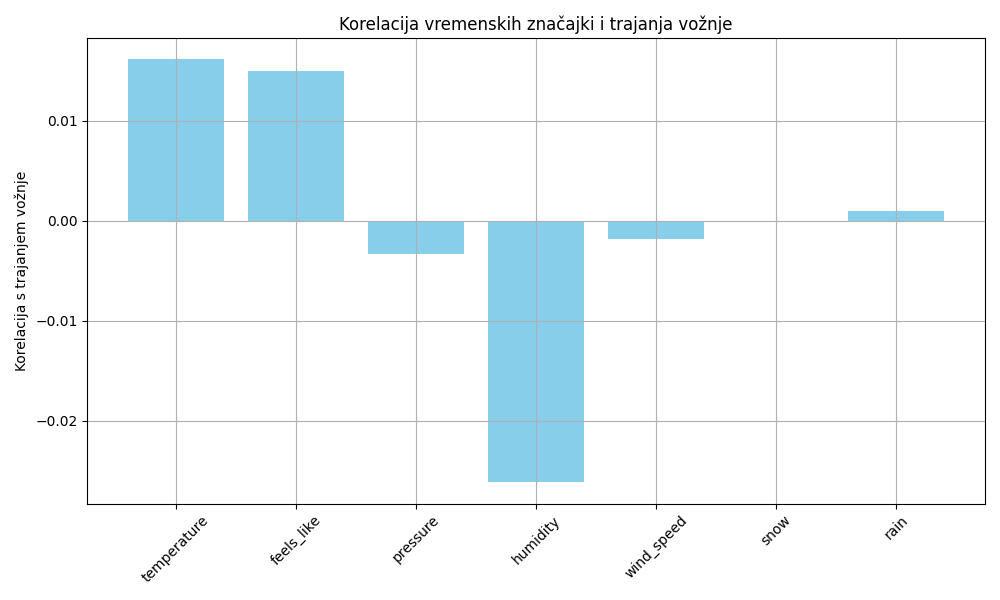
\includegraphics[width=\textwidth]{Figures/vrijeme_korelacija.png}
		\caption{Korelacija vremenskih značajki i trajanja vožnje}
		\label{fig:korelacije_vrijeme}
	\end{minipage}
	\hfill
	\begin{minipage}{0.48\textwidth}
		\centering
		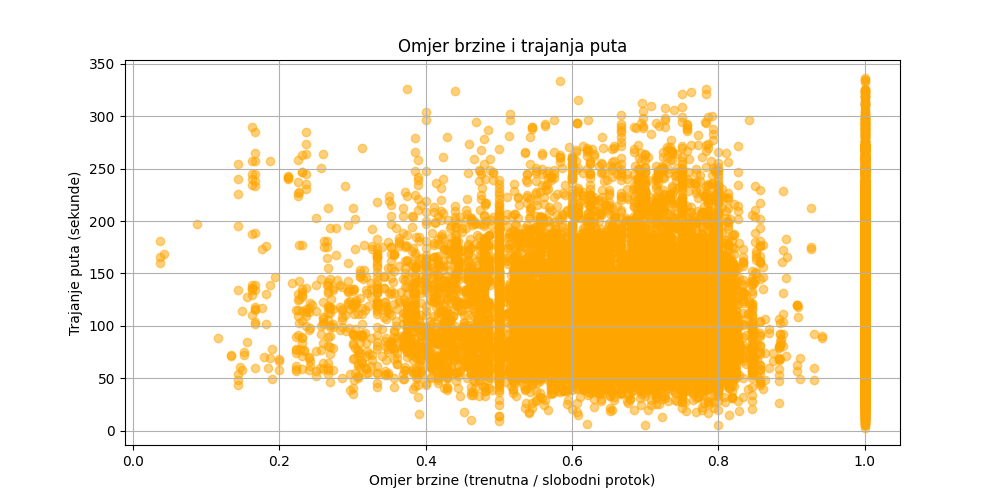
\includegraphics[width=\textwidth]{Figures/brzina_trajanje.png}
		\caption{Utjecaj brzine na trajanje puta}
		\label{fig:brzina_trajanje}
	\end{minipage}
\end{figure}

%--- ZAKLJUČAK / CONCLUSION ----------------------------------------------------
\chapter{Zaključak}
\label{pog:zakljucak}
U ovom seminarskom radu prikazan je jedan mogući primjer sustava koji bi se mogao koristiti za praćenje javnog gradskog prijevoza i ostvarivanje predikcija dolazaka prijevoza. Takav sustav mogao bi se dalje implementirati unutar korisničke aplikacije koja bi omogućila pristup ovim informacijama široj javnosti, čime bi se unaprijedilo iskustvo i planiranje putovanja korisnika javnog prijevoza. Primjena neuronske mreže u ovom sustavu pokazala se kao dobar izbor, jer je omogućila relativno precizne i pouzdane predikcije. S obzirom na ograničenja rada, koja se prvenstveno odnose na veličinu i raznolikost skupa podataka – budući da je prikupljanje provedeno u relativno kratkom vremenskom razdoblju i s ograničenim resursima (pristup API-ju) - za budući rad i razvoj takvog sustava potrebno je raditi na proširenju i točnosti dostupnog skupa podataka te dodatna optimizacija neuronske mreže radi povećanja učinkovitosti i preciznosti modela.
Zaključno, rad potvrđuje potencijal primjene umjetne inteligencije u unapređenju javnog gradskog prijevoza, što može doprinijeti većem zadovoljstvu korisnika i učinkovitijem prometnom sustavu.

%--- LITERATURA / REFERENCES ---------------------------------------------------

% Literatura se automatski generira / References are automatically generated
% Upiši ime BibTeX datoteke bez .bib nastavka / Enter the name of the BibTeX file without .bib extension
\nocite{*}
\bibliography{literatura}


\end{document}
